\section{Lois discrètes}
\begin{figure}[H]
    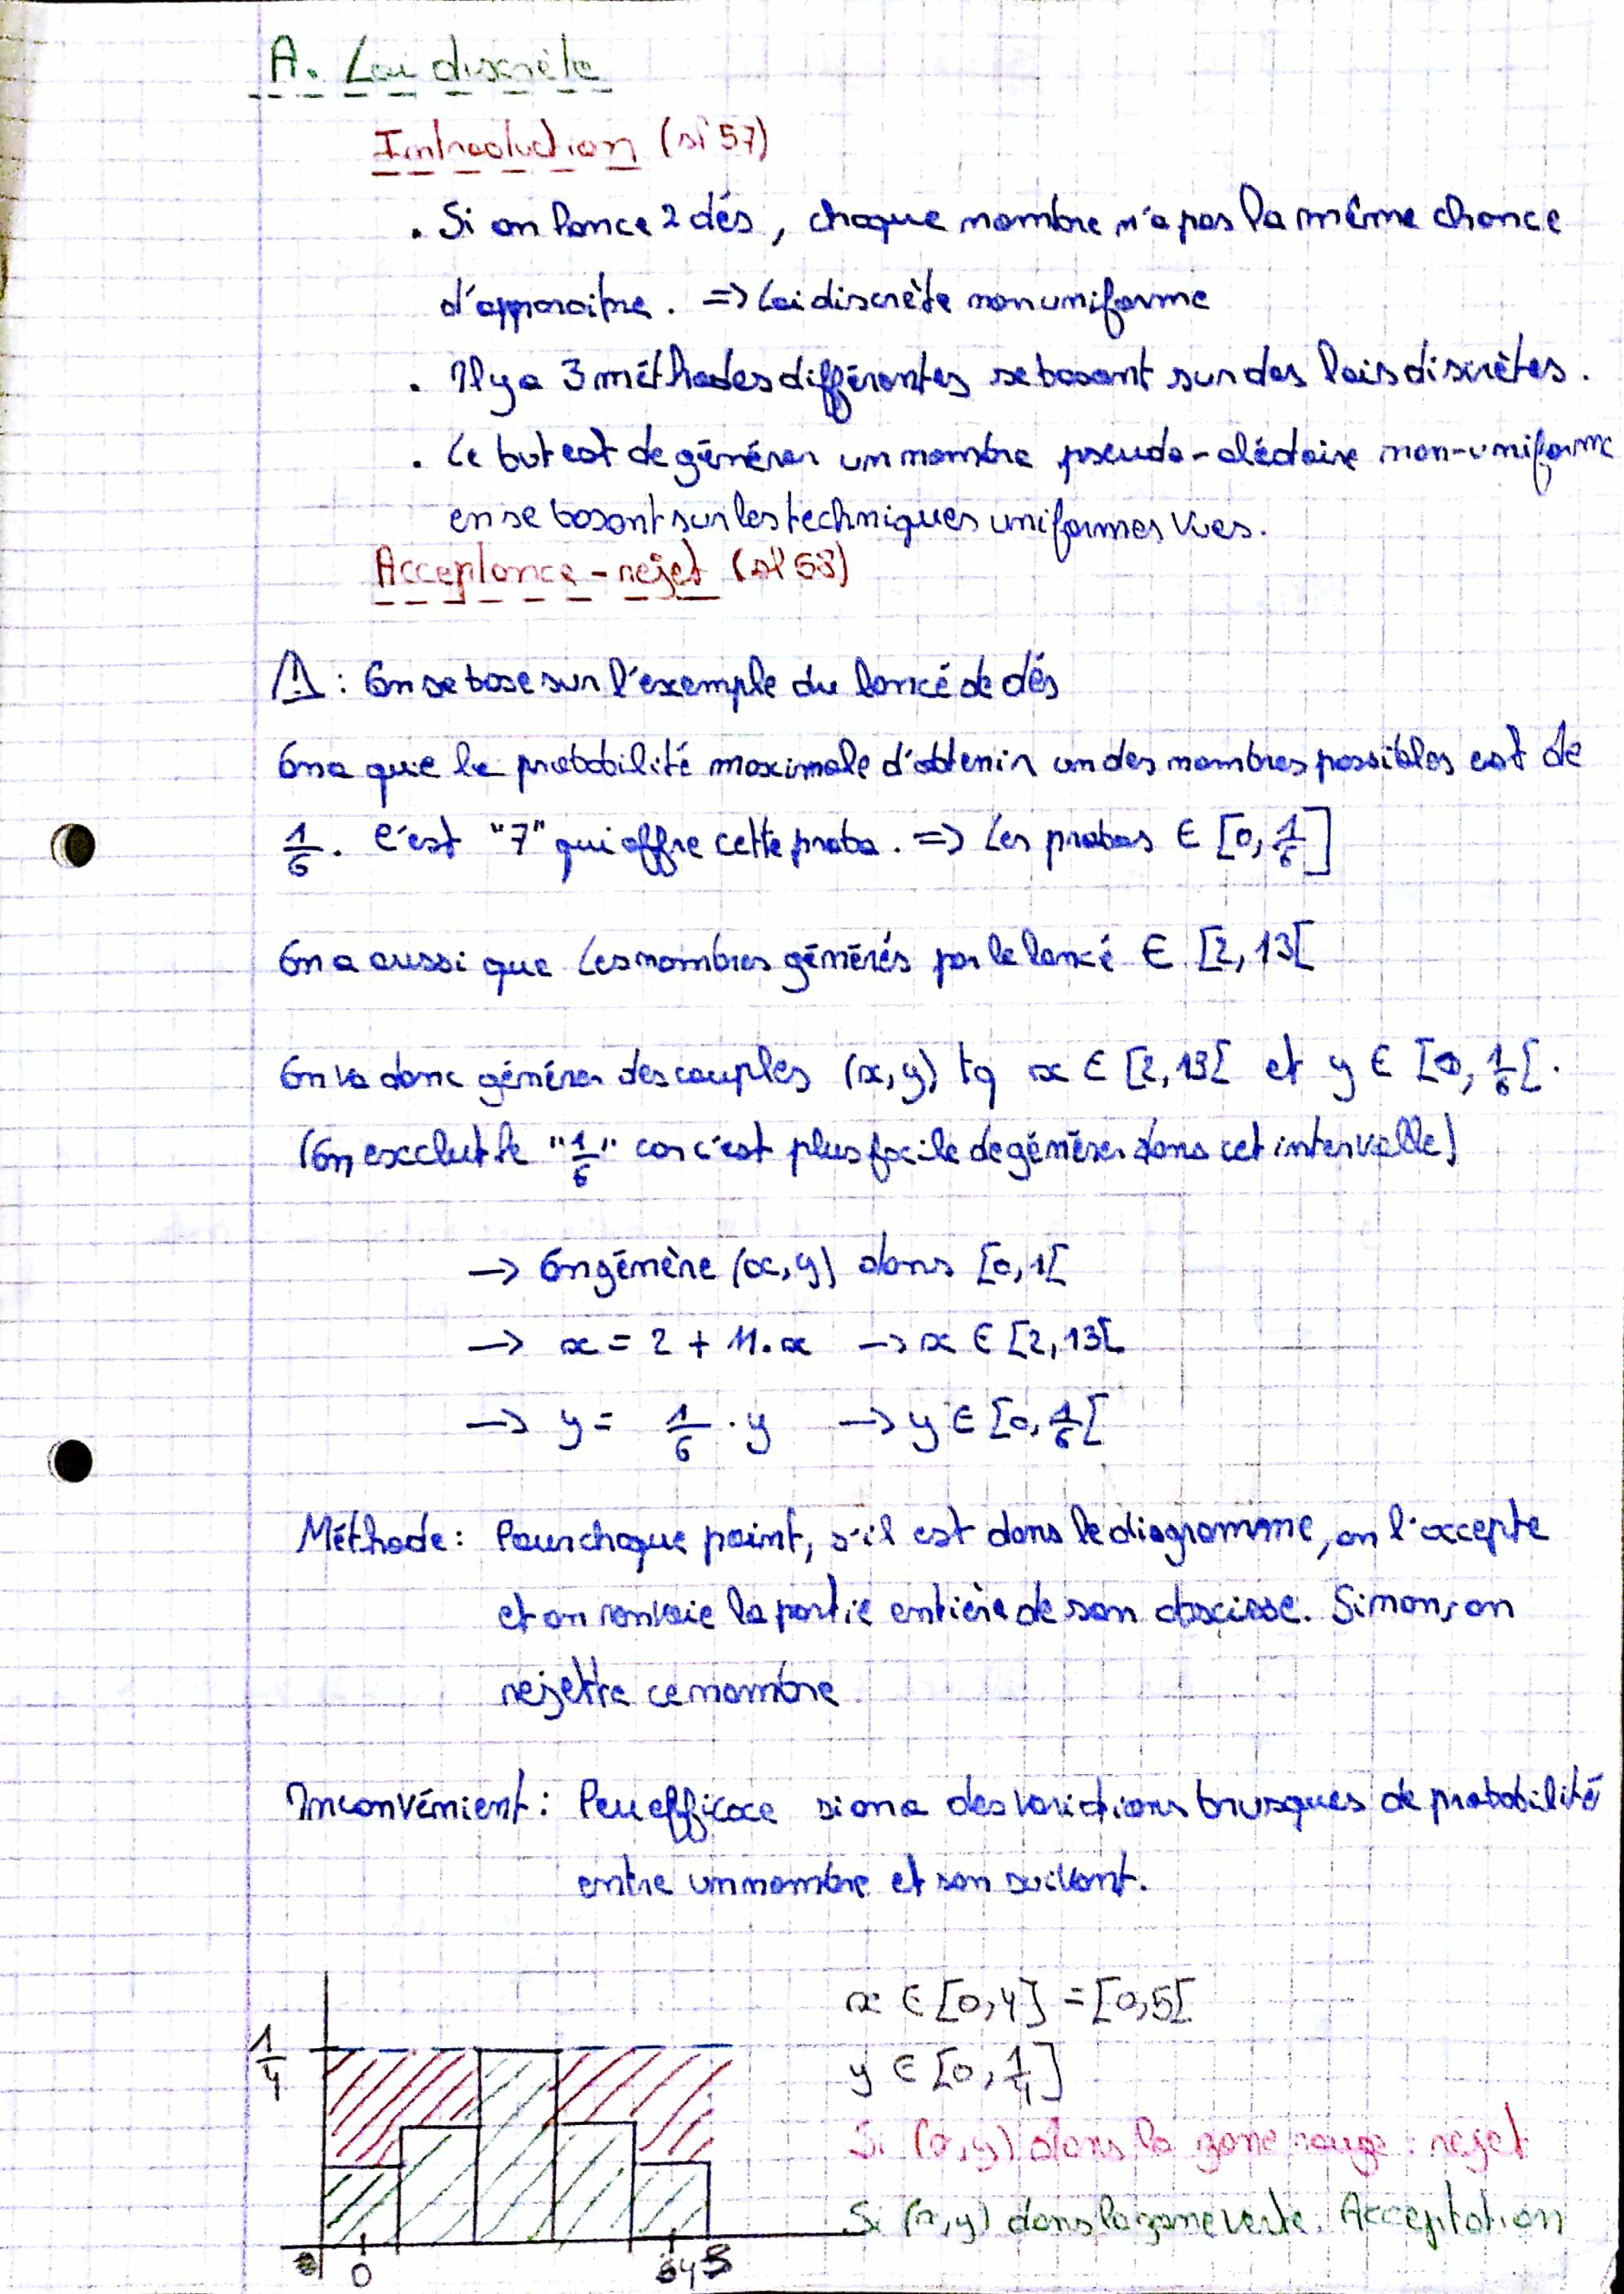
\includegraphics[height=\textheight-1.16cm]{Jonathan(1)}
\end{figure}
\begin{figure}[H]
    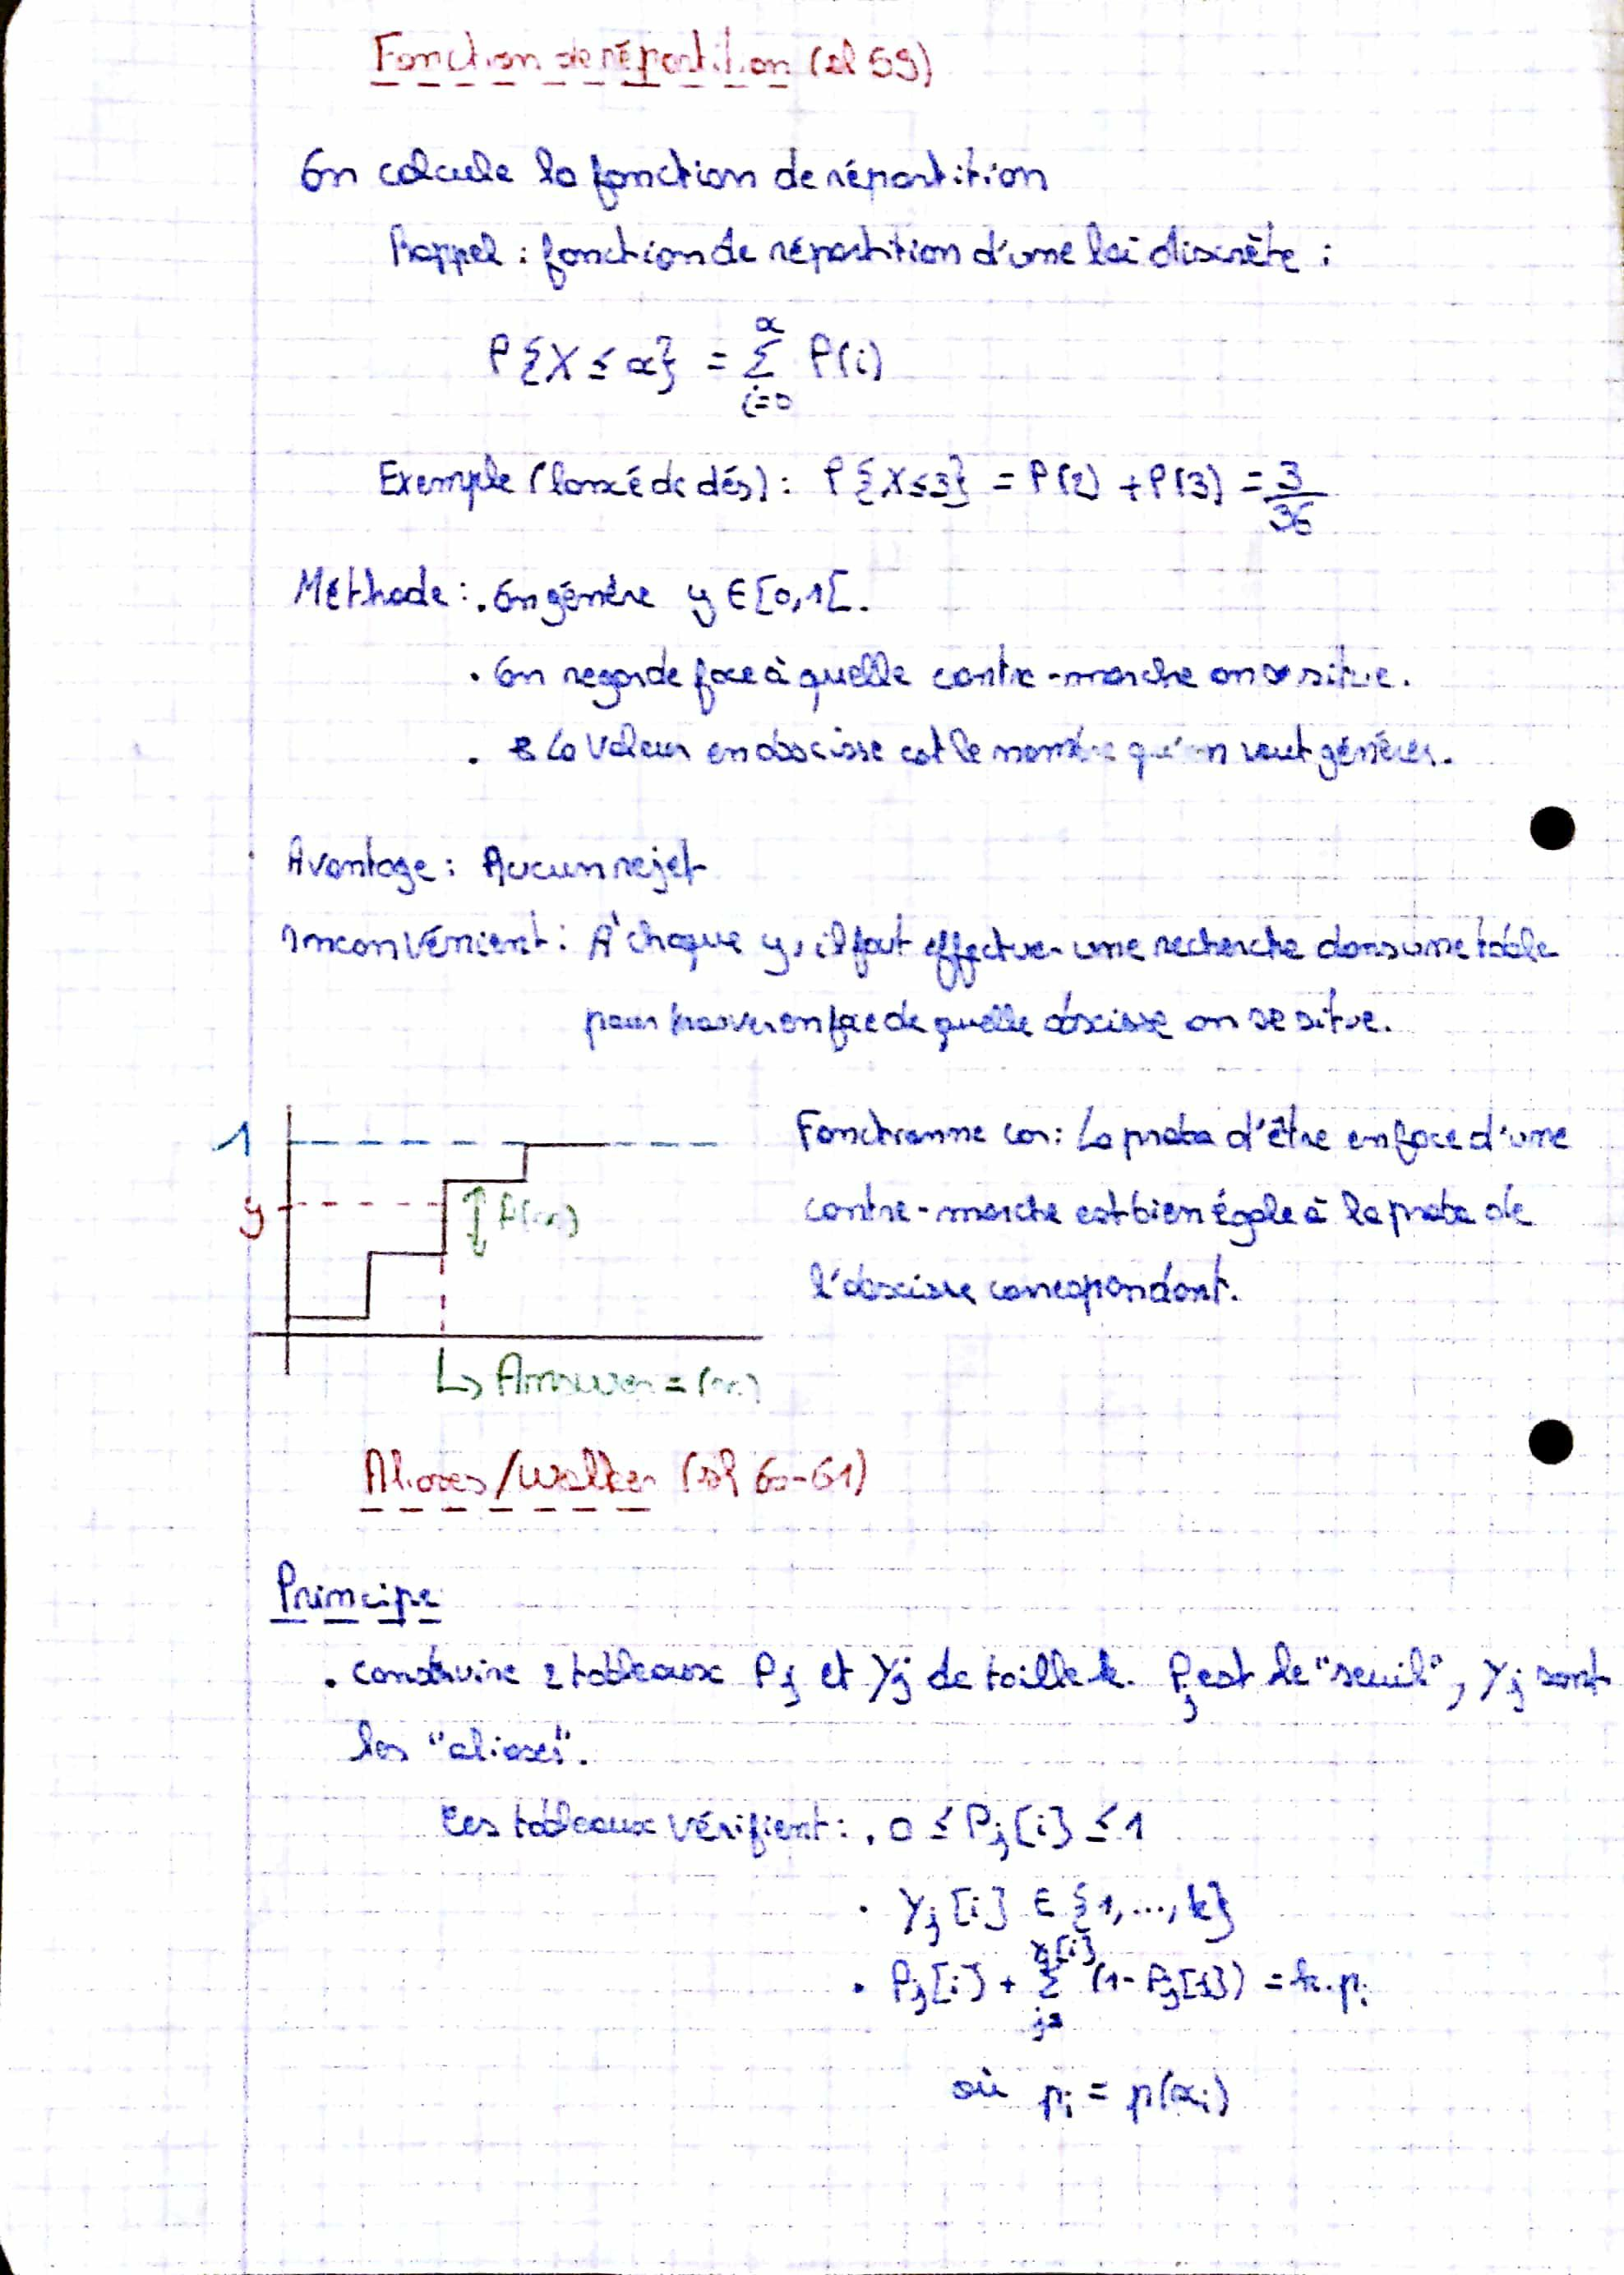
\includegraphics[width=\textwidth]{Jonathan(2)}
\end{figure}
\begin{figure}[H]
    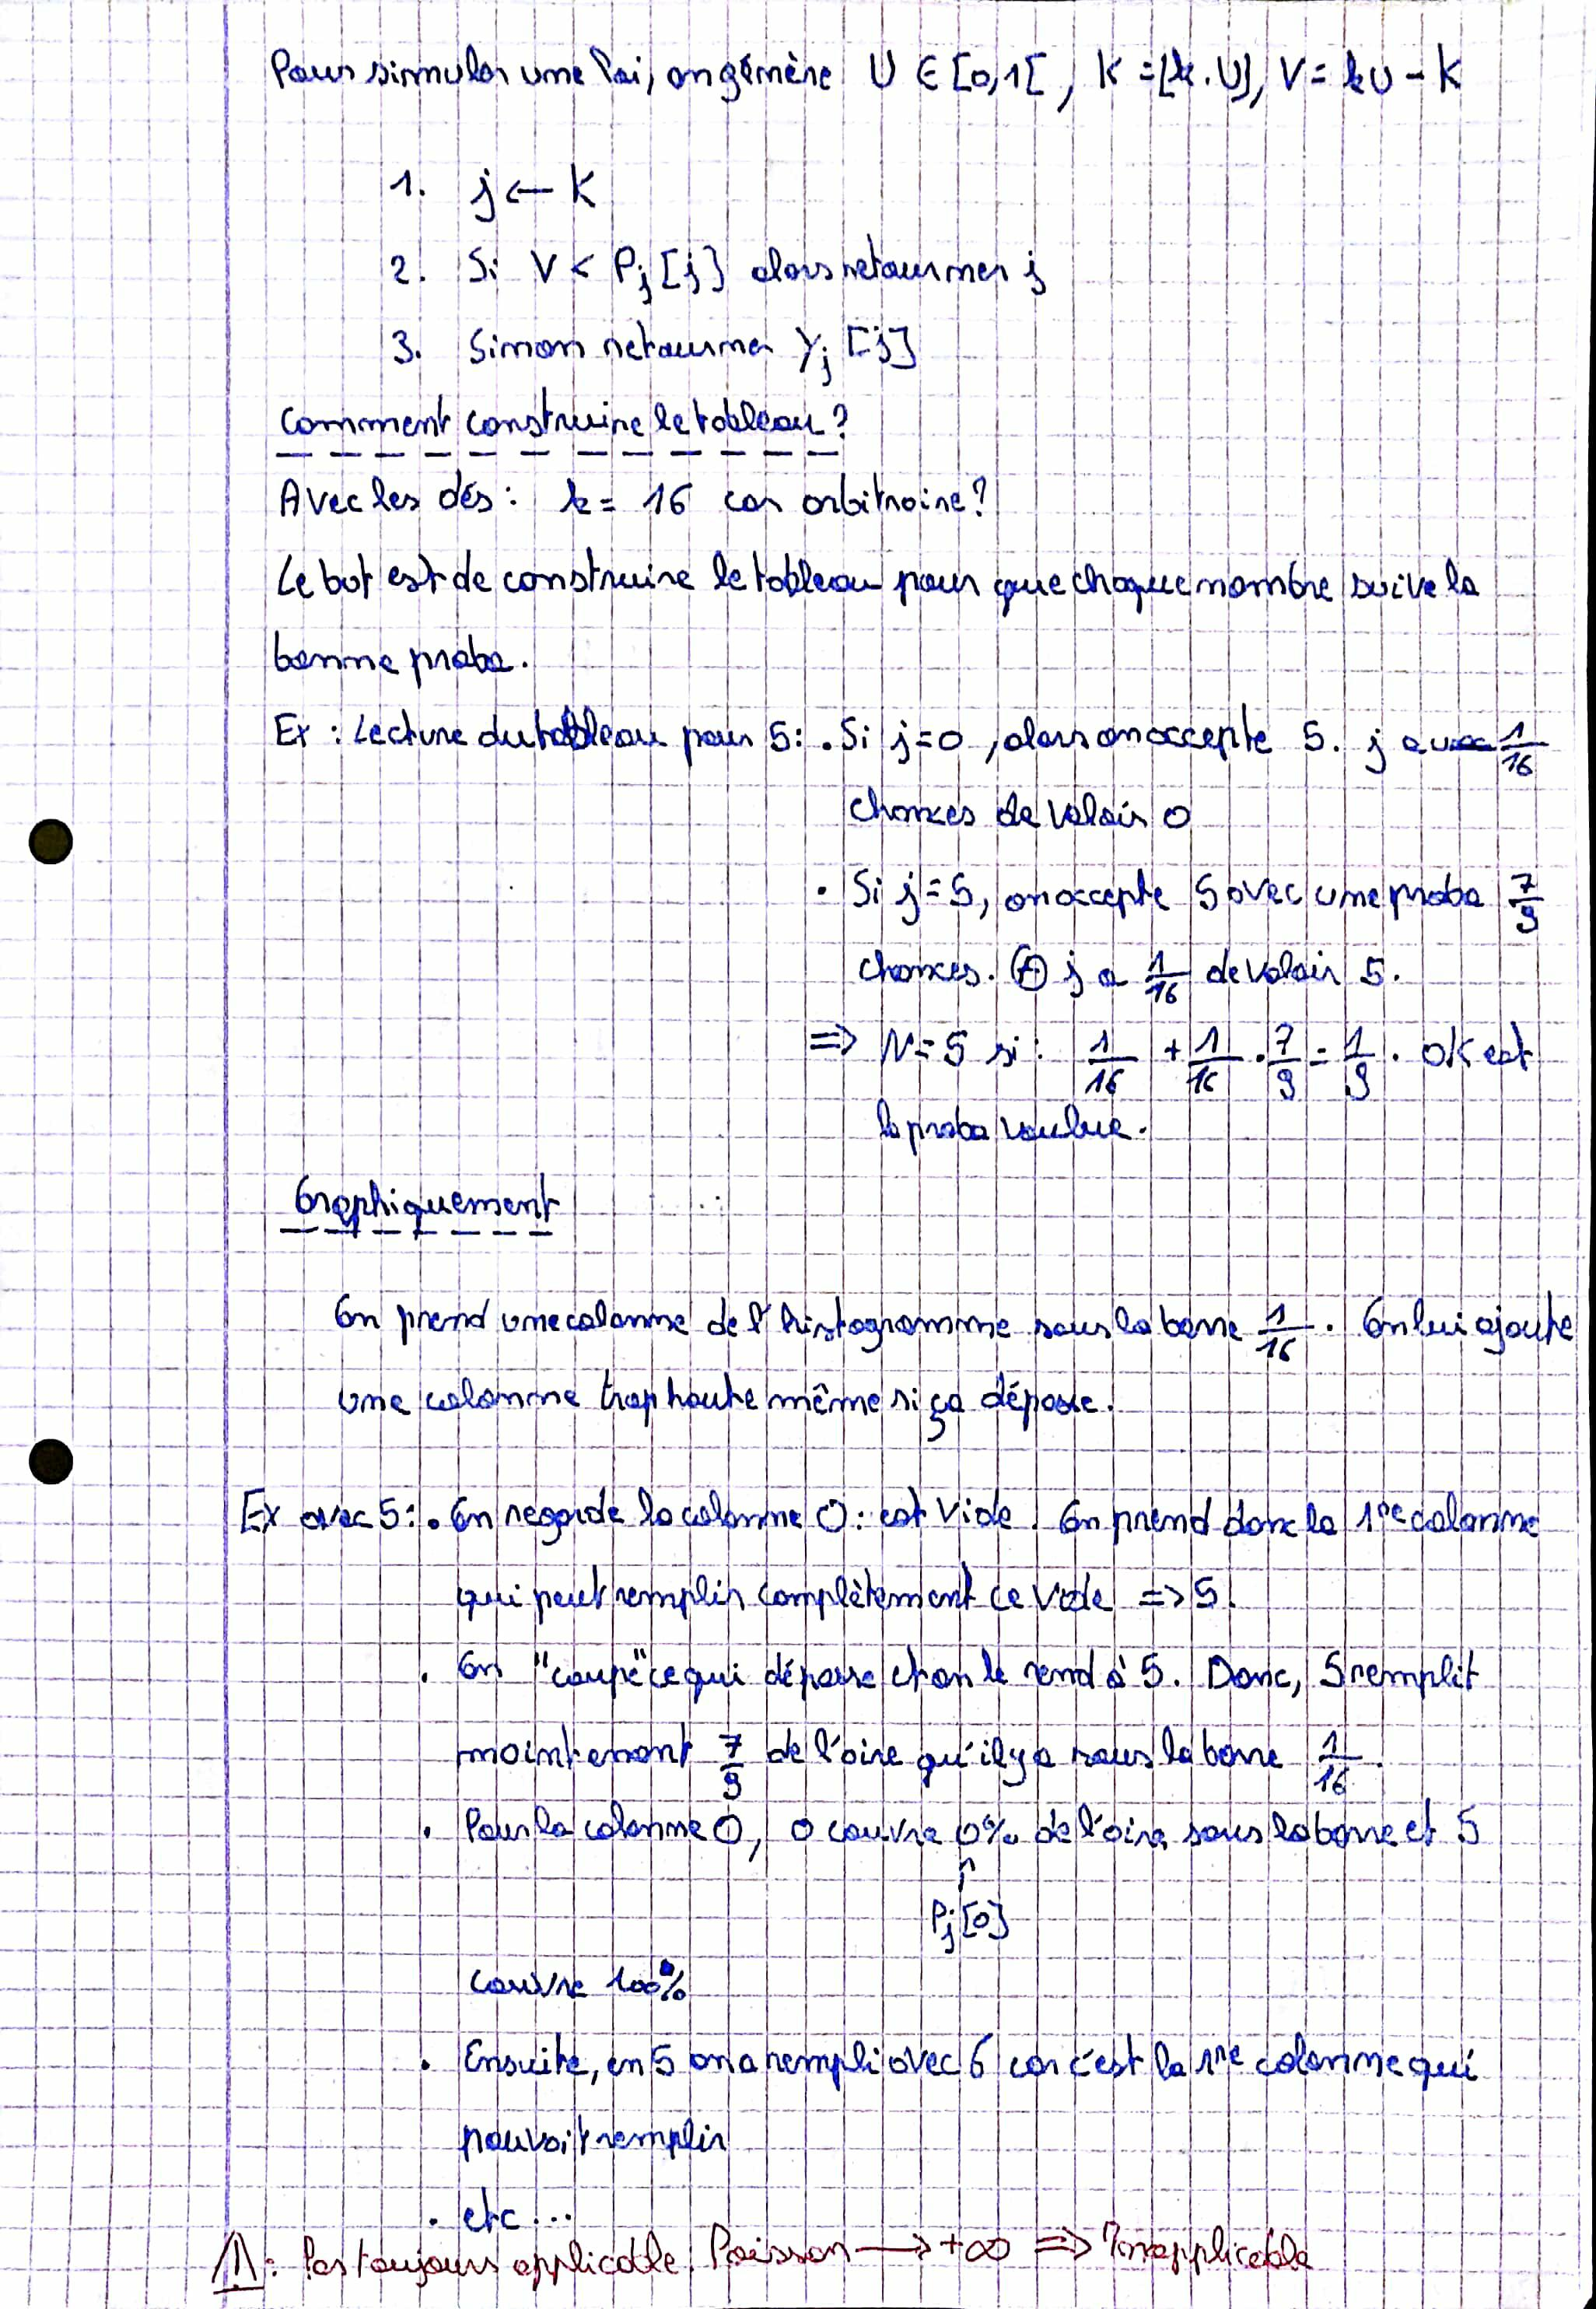
\includegraphics[width=\textwidth]{Jonathan(3)}
\end{figure}
\section{Lois continues}
\subsection{Acceptance-rejet et inversion de la fonction de répartition}
\begin{figure}[H]
    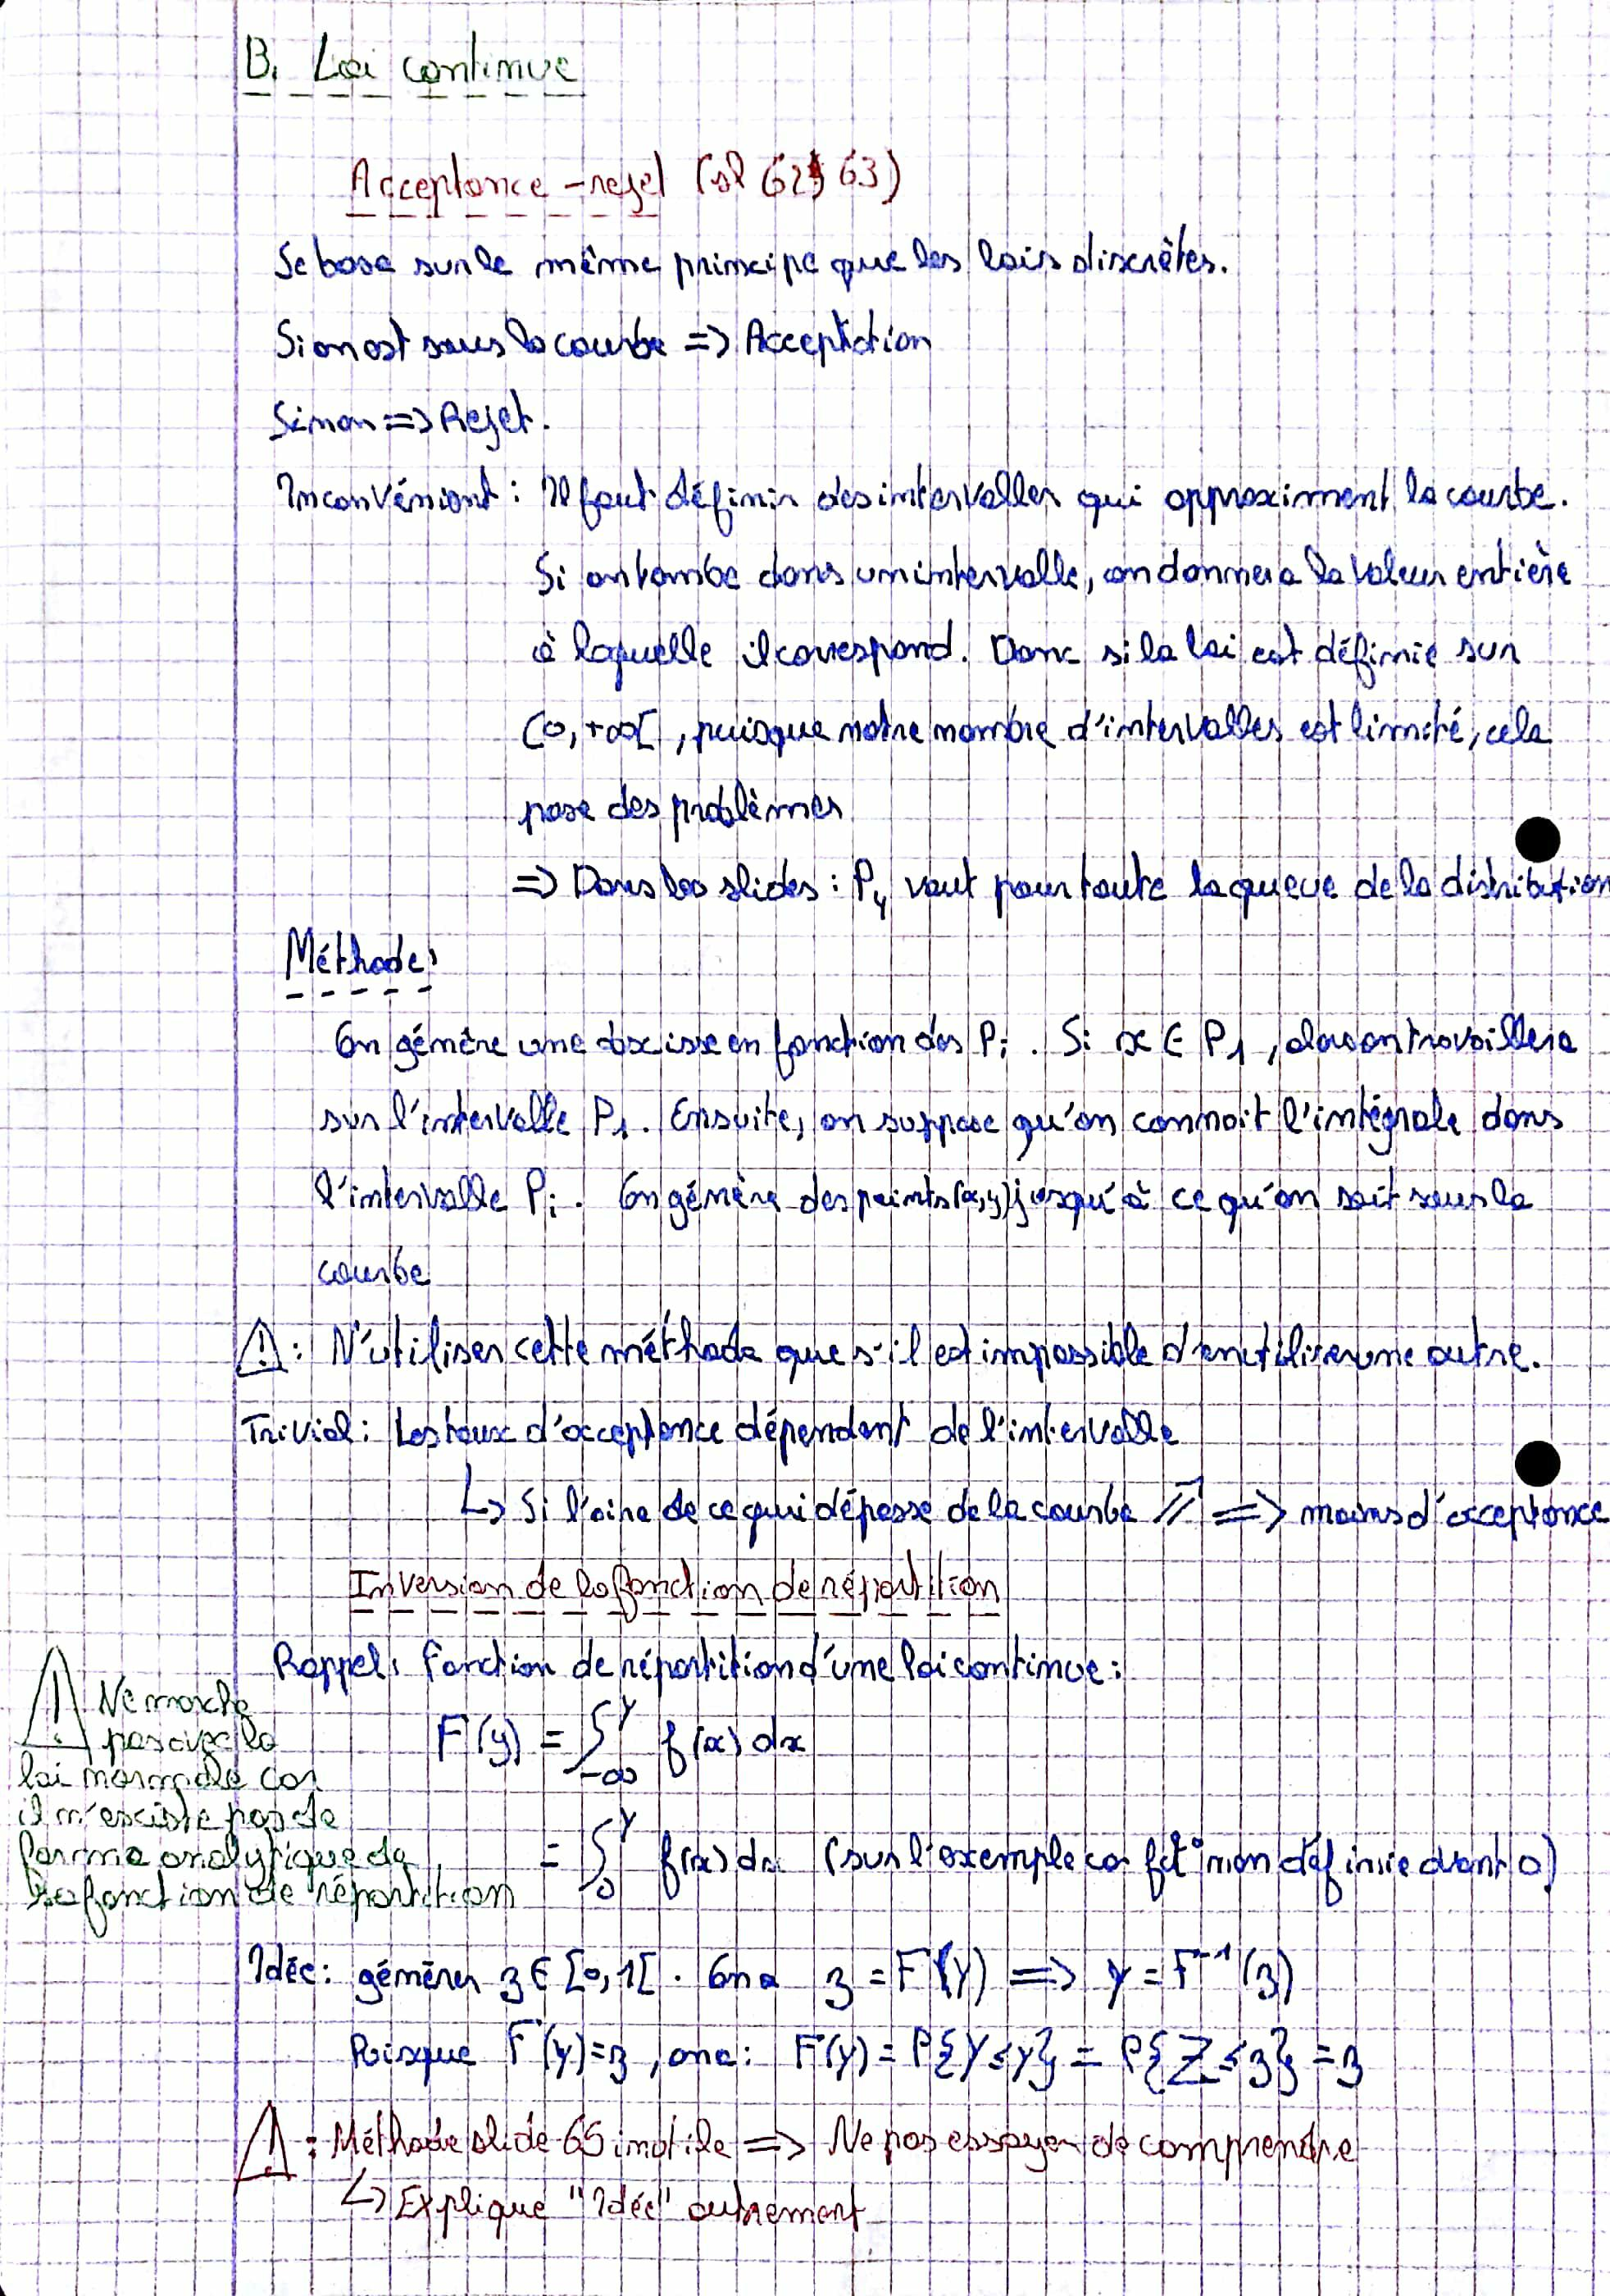
\includegraphics[width=\textwidth-1.16cm]{Jonathan(4)}
\end{figure}
\begin{figure}[H]
    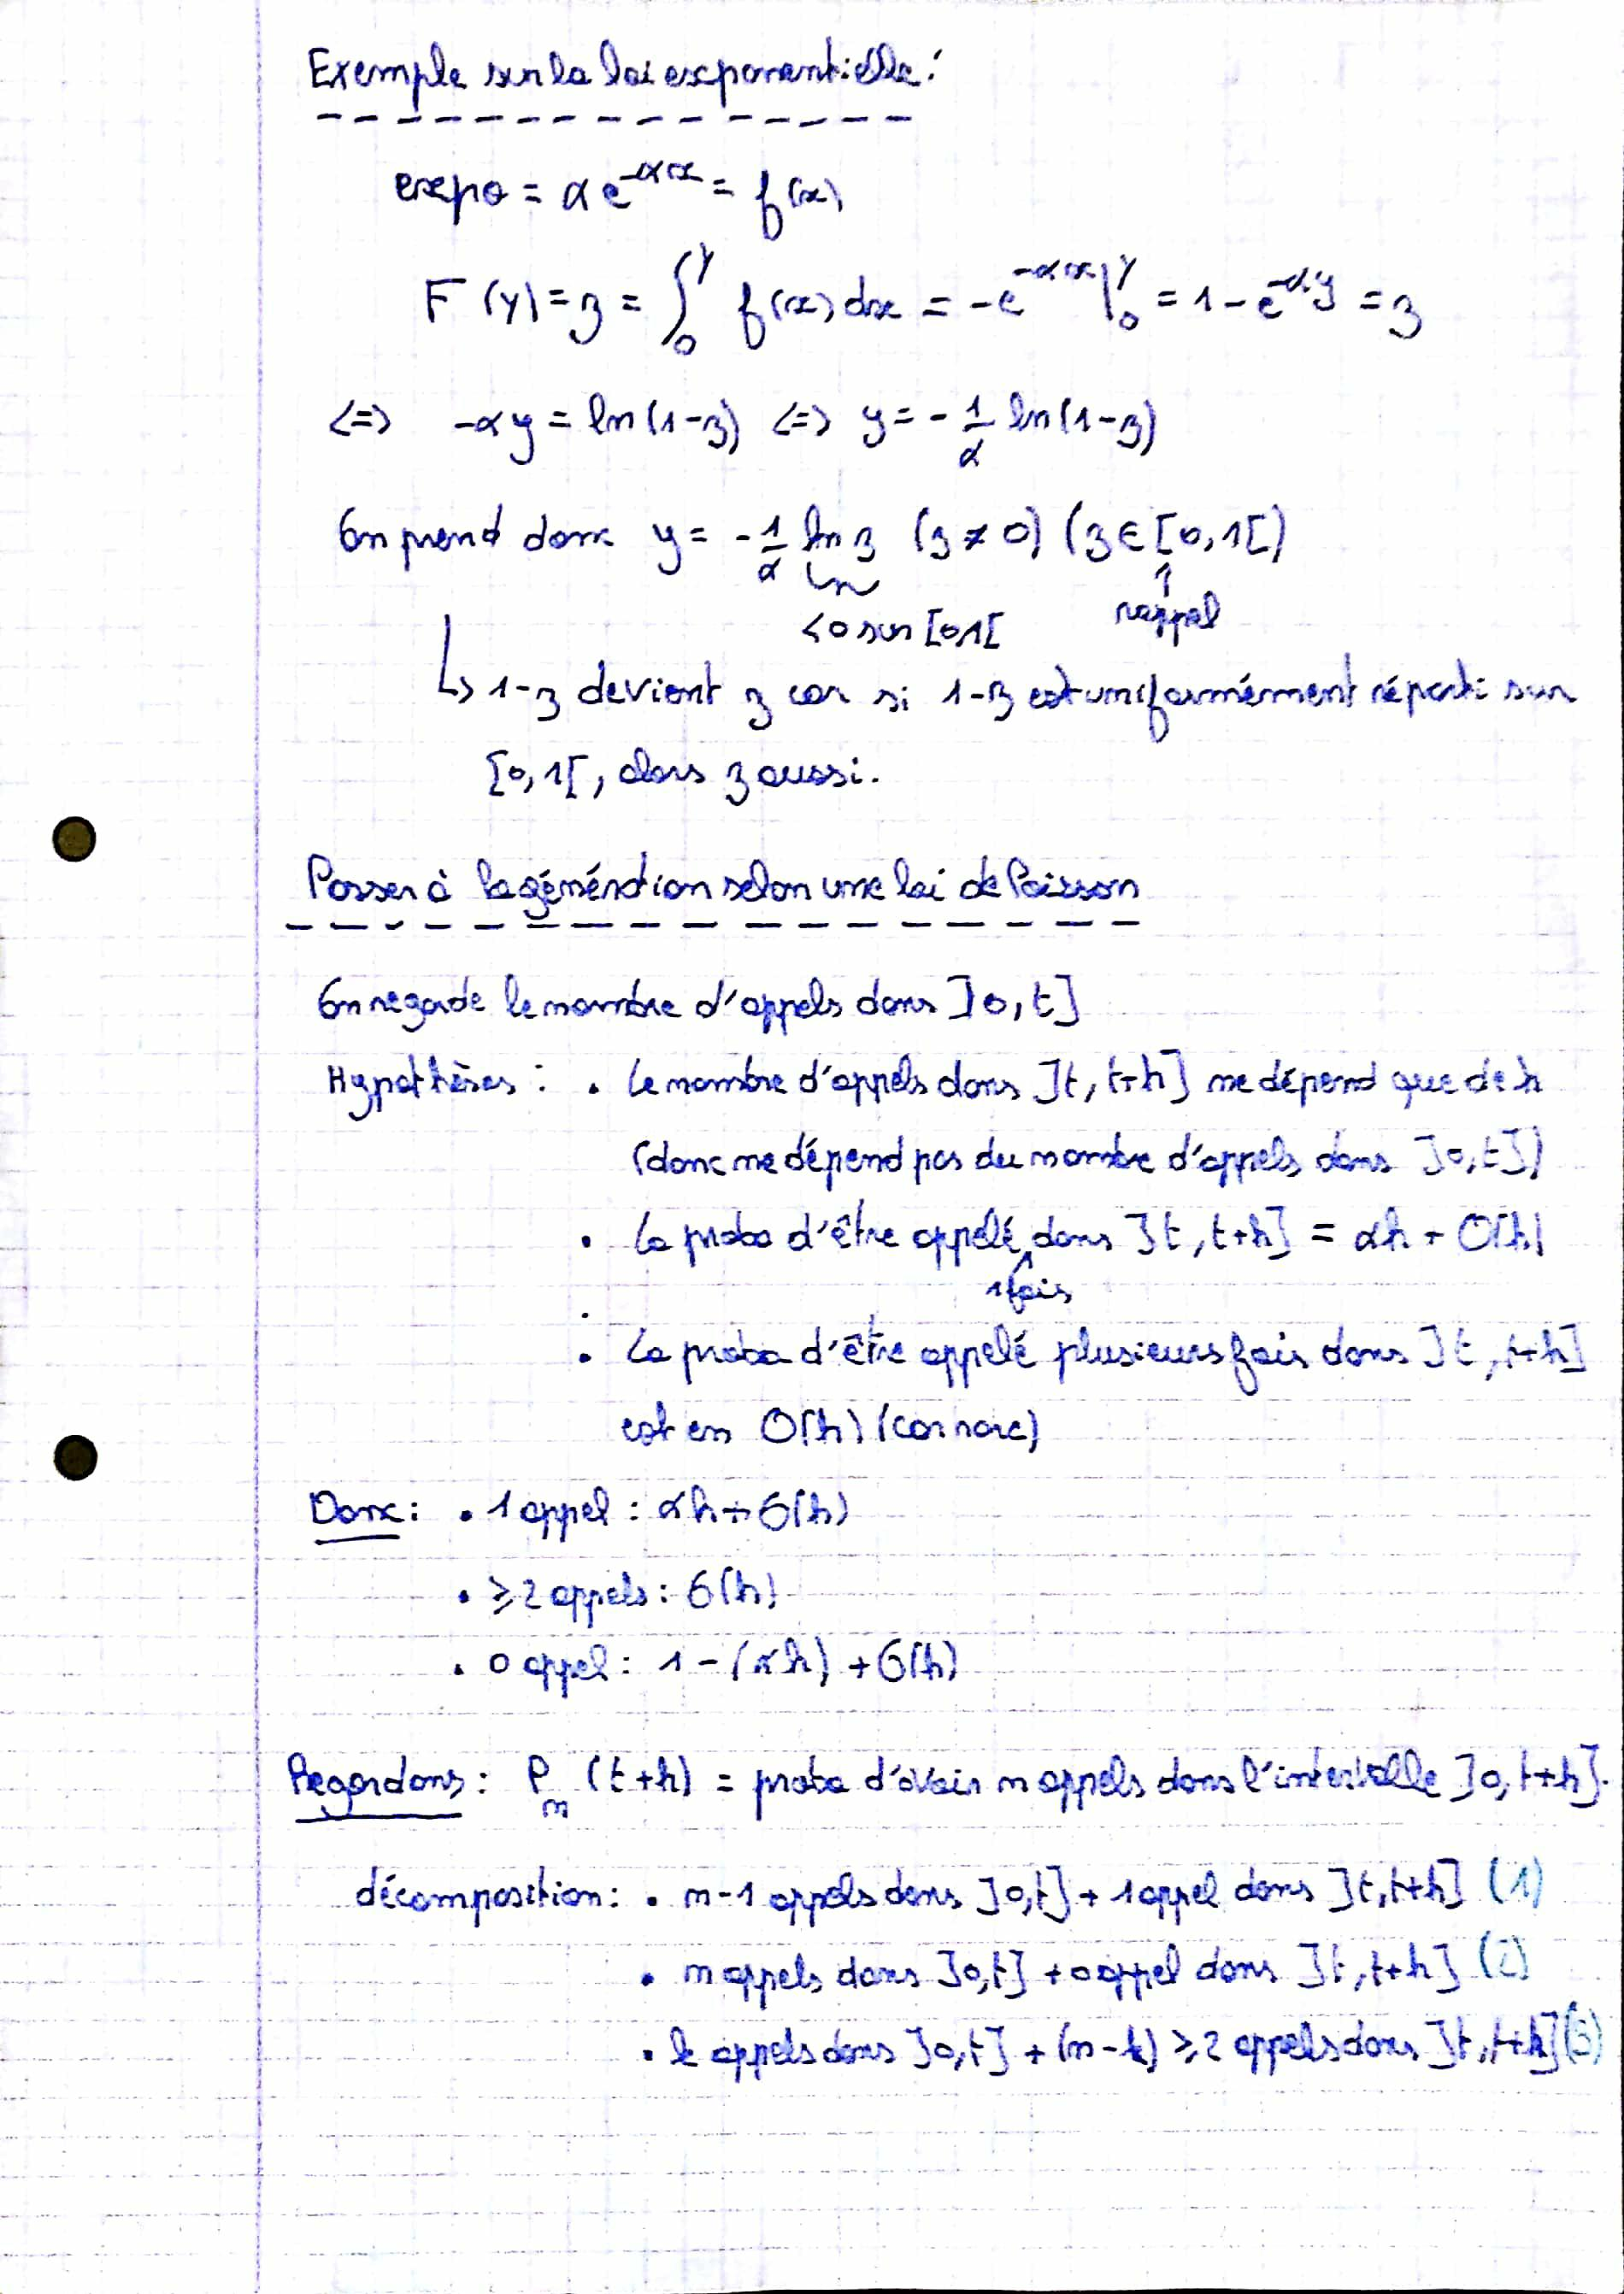
\includegraphics[width=\textwidth]{Jonathan(5)}
\end{figure}
\begin{figure}[H]
    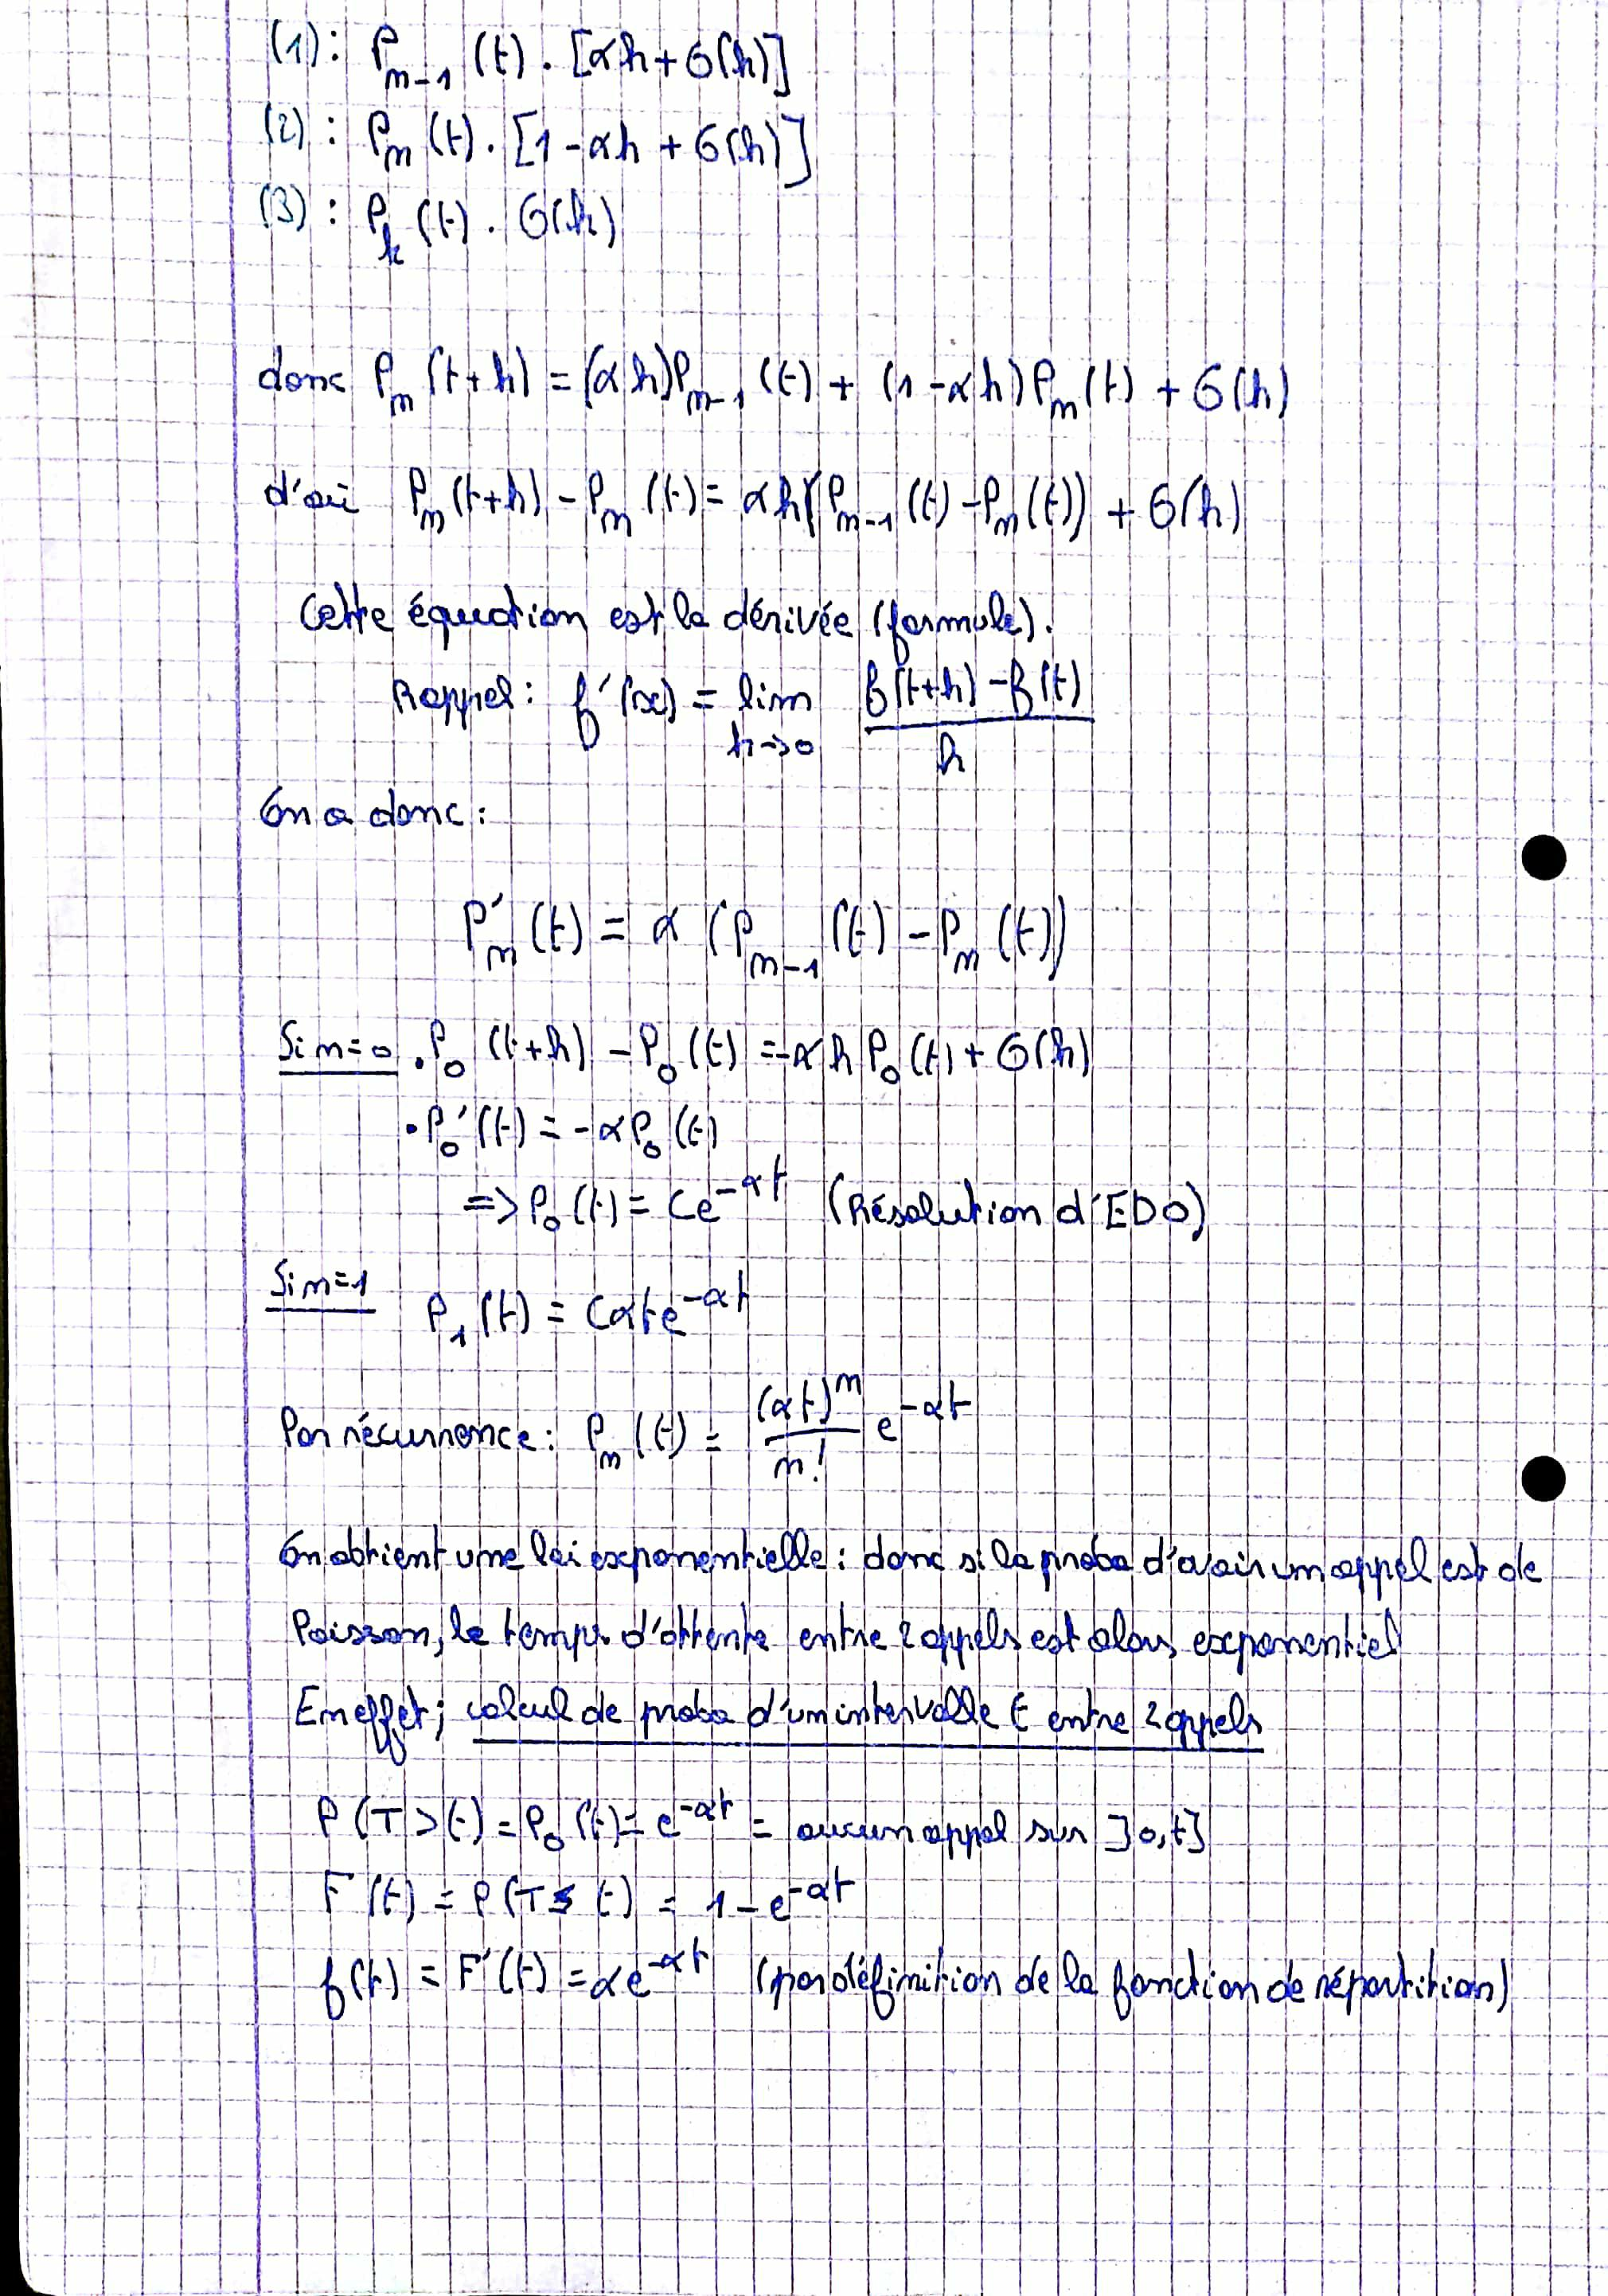
\includegraphics[width=\textwidth]{Jonathan(6)}
\end{figure}
\begin{figure}[H]
    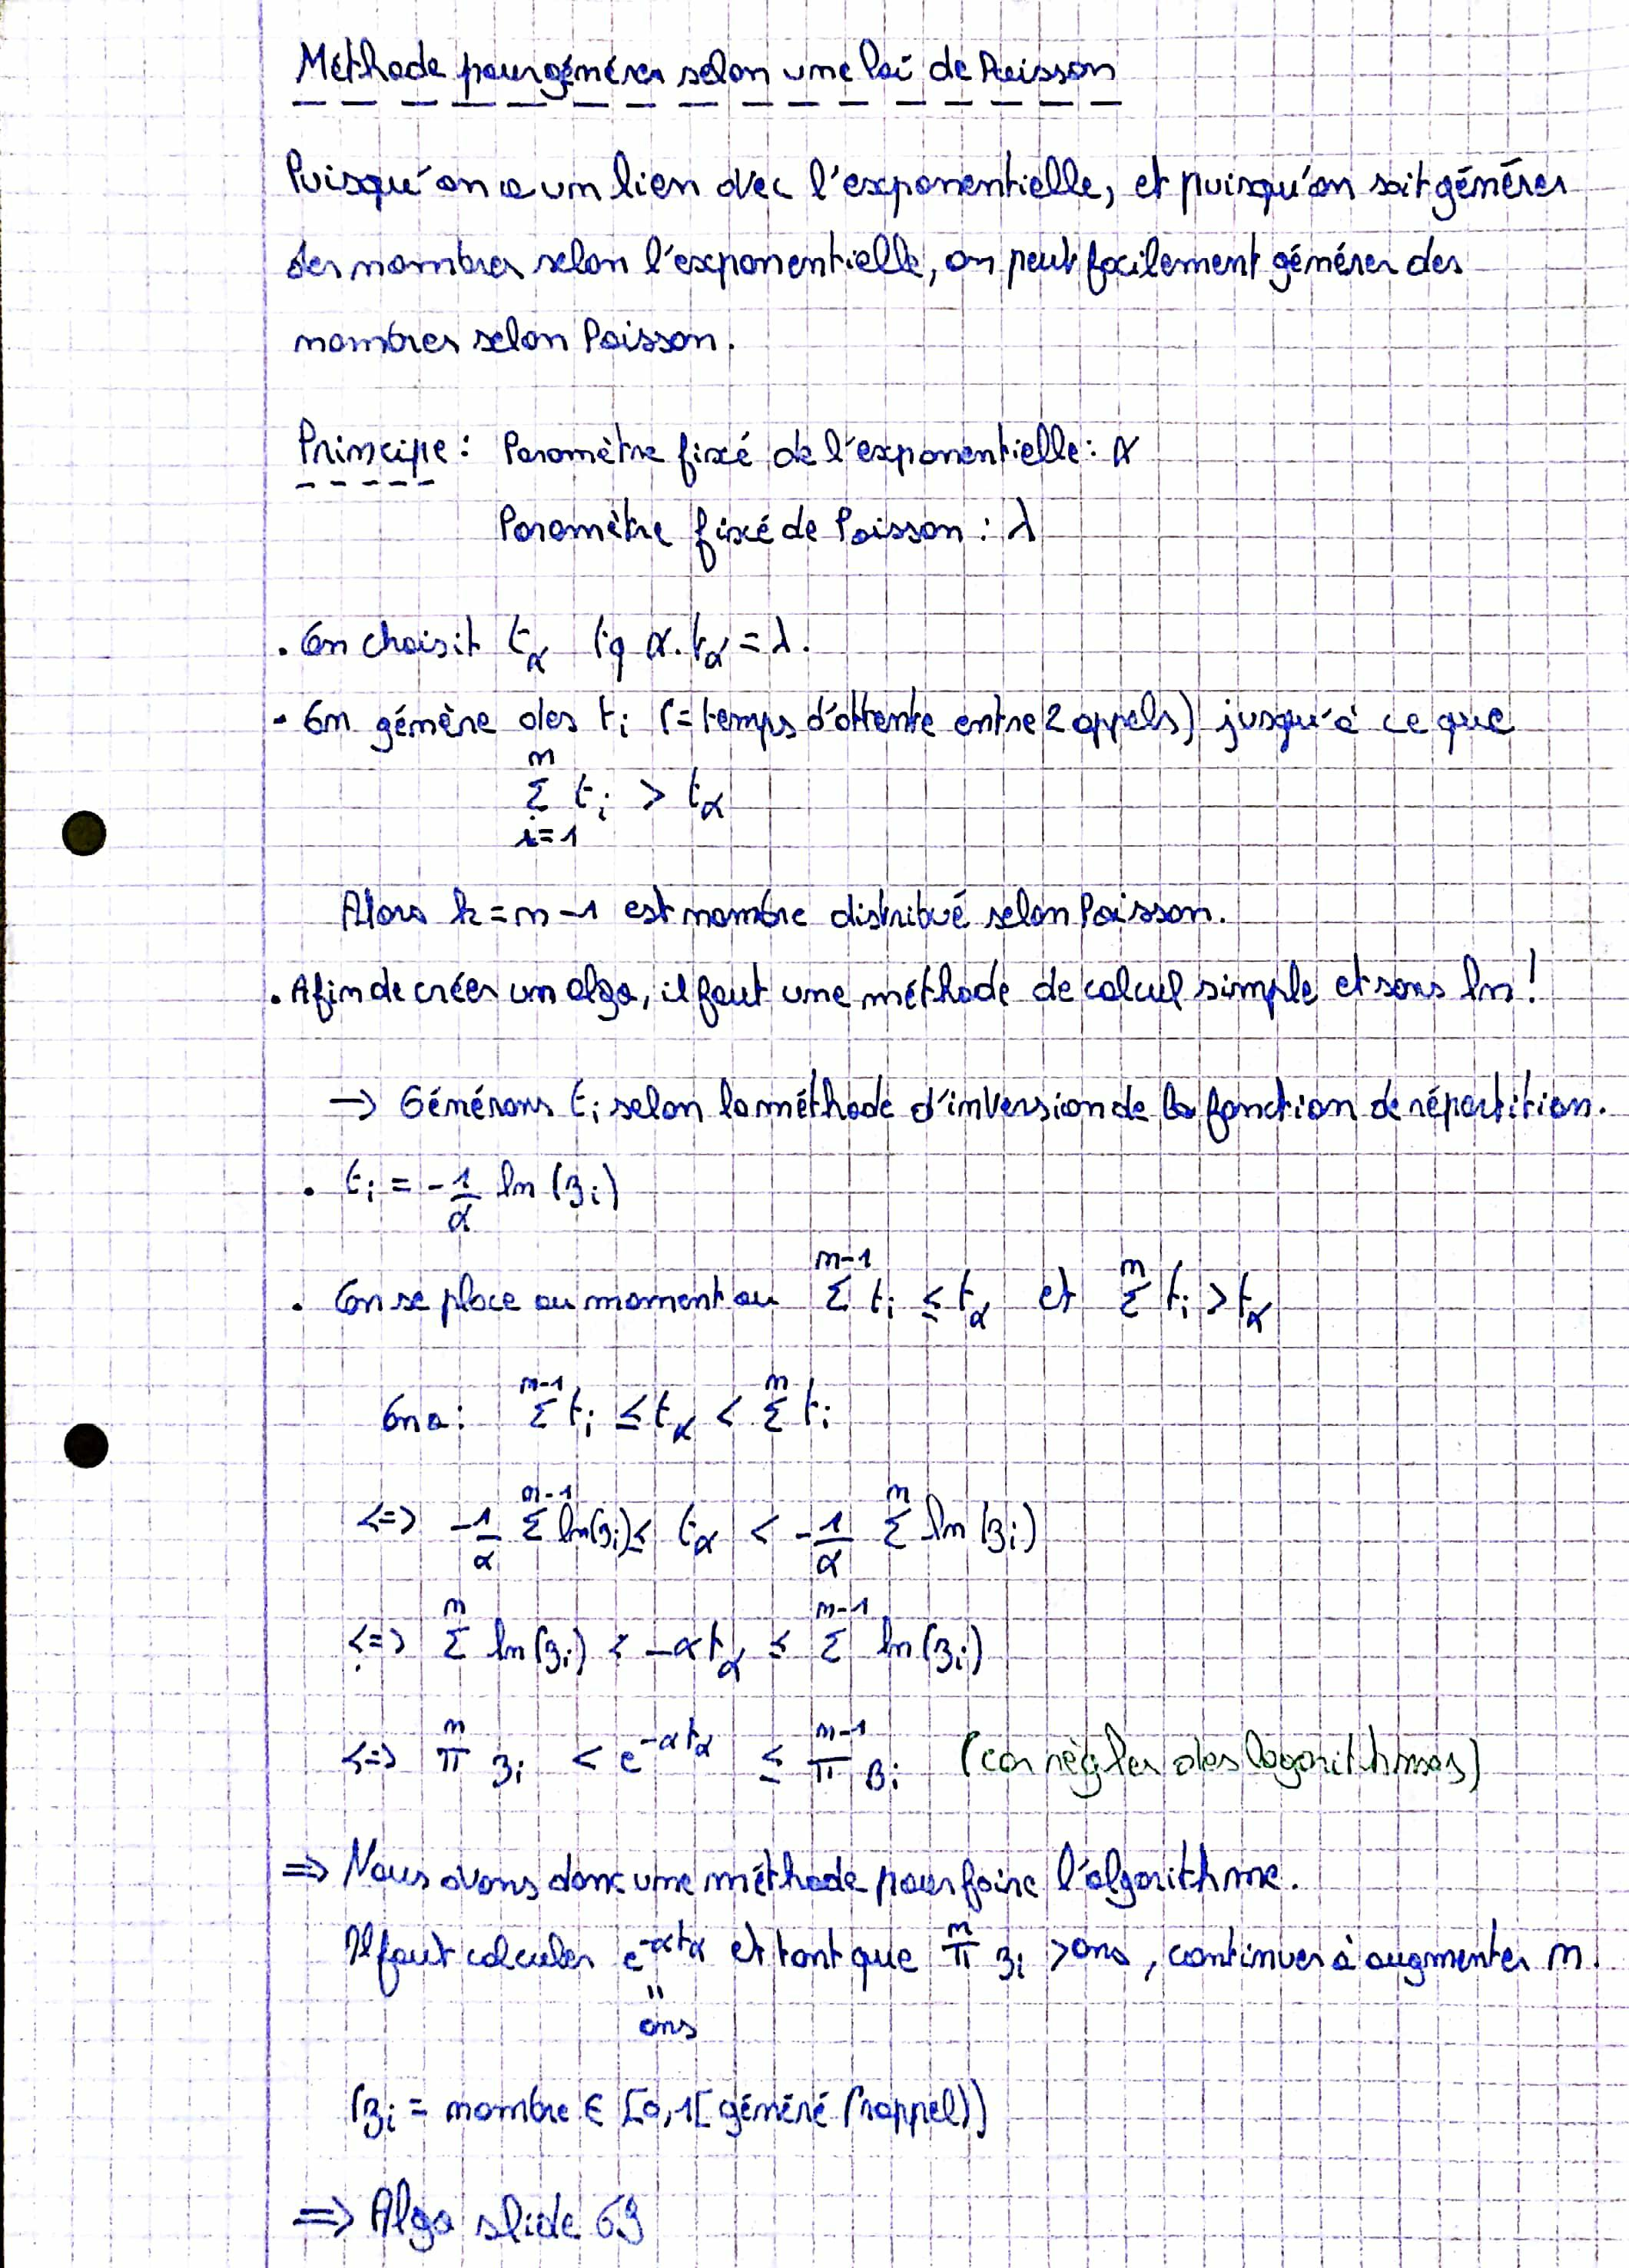
\includegraphics[width=\textwidth]{Jonathan(7)}
\end{figure}